\section{Process and methodology}
\label{sec:process-approach}
	
	The main effort of the current stage of the project is to develop a formal ontology. This corresponds to Step \ref{step:5} of the process described in \cite[3--15]{d2.01-2017} and repeated in Section \ref{sec:context}.	
	
	This section expands and addresses in detail the process of defining and implementing an OWL eProcurement ontology. The underlying assumption is that the conceptual data model developed at Step \ref{step:3} serves as an input for the creation of the ontology, and that this process shall be automatic. 
	
	In addition to producing the ontology as an artefact, we also needs to validates its fitness to represent existing data and test whether the functional and non-functional requirements are respected. Figure \ref{fig:process-overview} depicts the sequence of steps as a BPMN process diagram \cite{bpmn-introduction}. 
	
	\begin{figure}[!ht]		
		\centering
		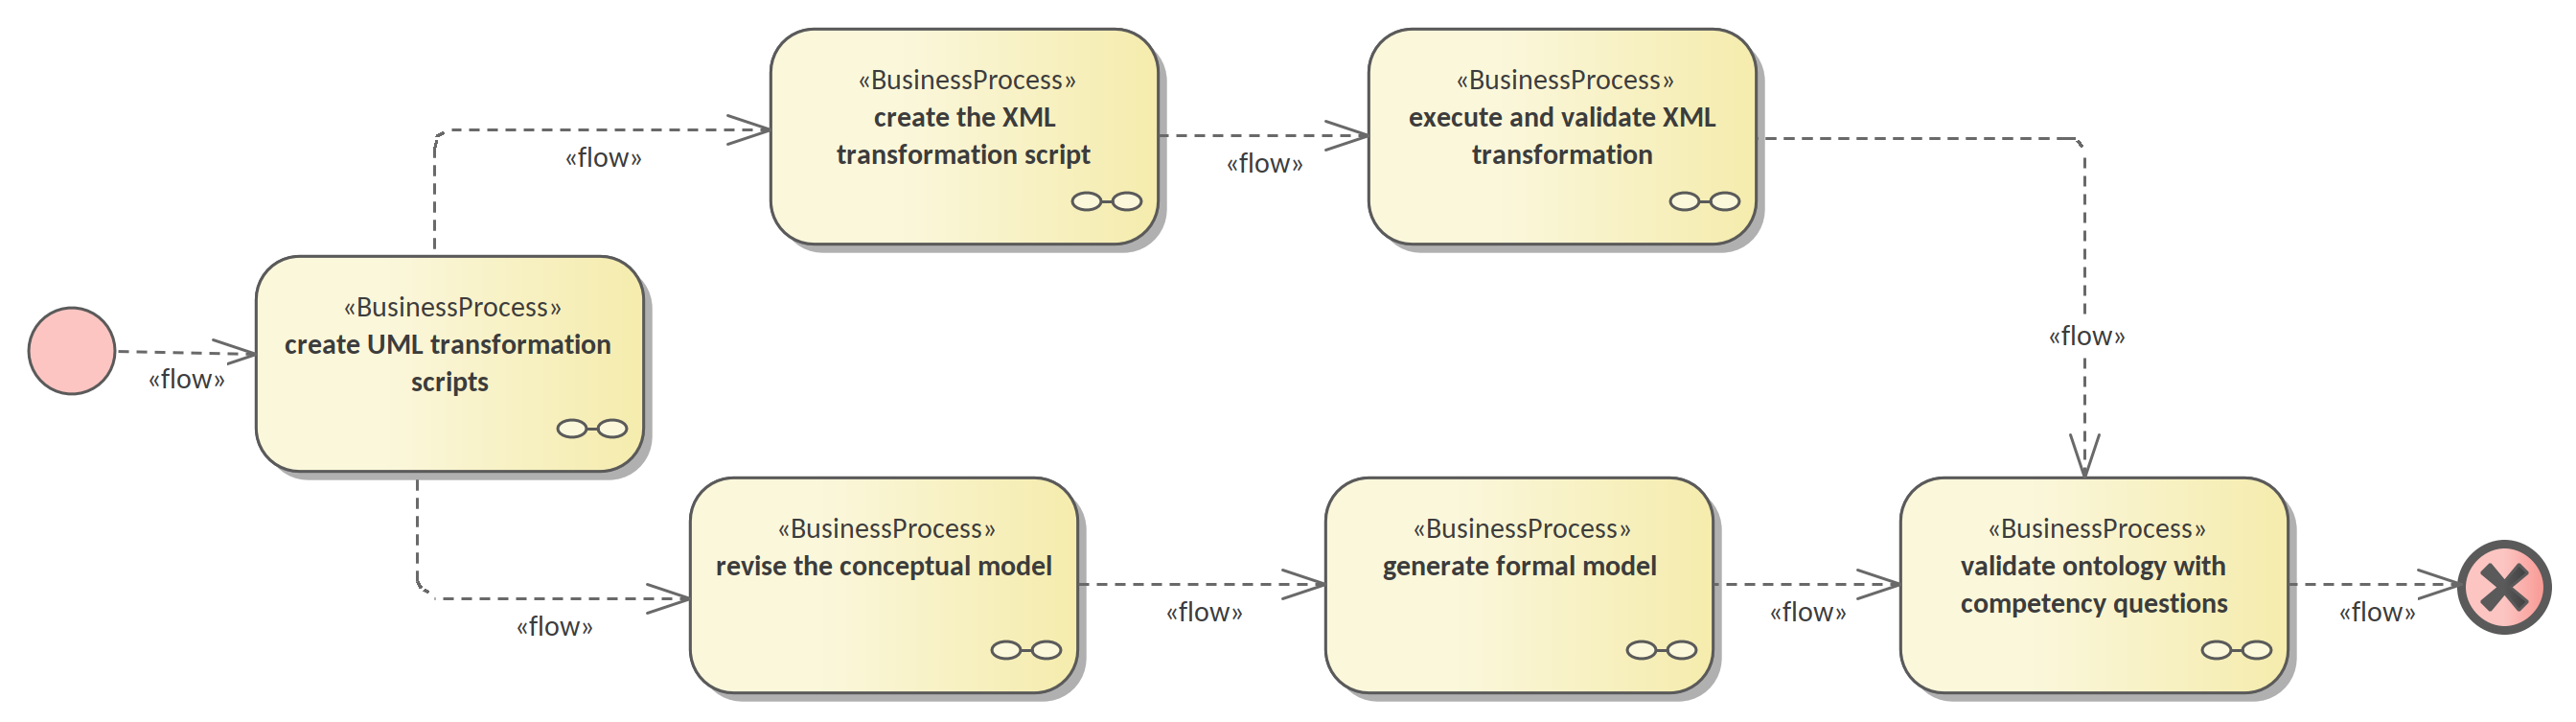
\includegraphics[width=\textwidth]{../img/processOverview.png}
		\caption{The main steps to implementing and validating the formal eProcurement ontology}
		\label{fig:process-overview}
	\end{figure}

	The conceptual model serves as the single source of truth, the process starts with development of a series of transformations scripts. The conceptual model needs to be adjusted in order to fit a set of UML modelling conventions \citep{costetchi2020b} making it suitable input for the transformation scripts. Provided that the conceptual model is conform, the transformation can be executed. Finally the validation of the formal ontology can be performed using the existing eProcurement data.
	
	
	%	after the creation of the UML transformation scripts, which also sets in place the ontology architecture, this document, and the UML conventions \citep{costetchi2020b}
	The existing eProcurement data needs to be transformed from XML into RDF format. So, in parallel, after the UML transformations are created and along with them, the ontology architecture and UML conventions, then a set of XML transformation scripts can be developed. Once they are ready, they need to be executed on previously selected datasets, to convert them into RDF data instantiating the formal ontology. Only then, when the datasets are available, the ontology can be validated. 
	
	The next subsections describe each of these six steps in more detail in order to provide rationale and introduce each artefact in part.
	
	\subsection{UML transformation scripts}
	\label{sec:uml-transformation}
	
	The process start with authoring two documents laying the foundations of the entire process: the ontology architecture and the UML modelling conventions \citep{costetchi2020b}. The main purpose of the ontology architecture (this document) specifications is to describe why the ontology is being built, what its intended uses are, who the end-users are, and which requirements the ontology should fulfil. Moreover, it states how the ontology should be structured in order to facilitate maintenance and usage patterns.
	
	
	\begin{figure}[!ht]		
		\centering
		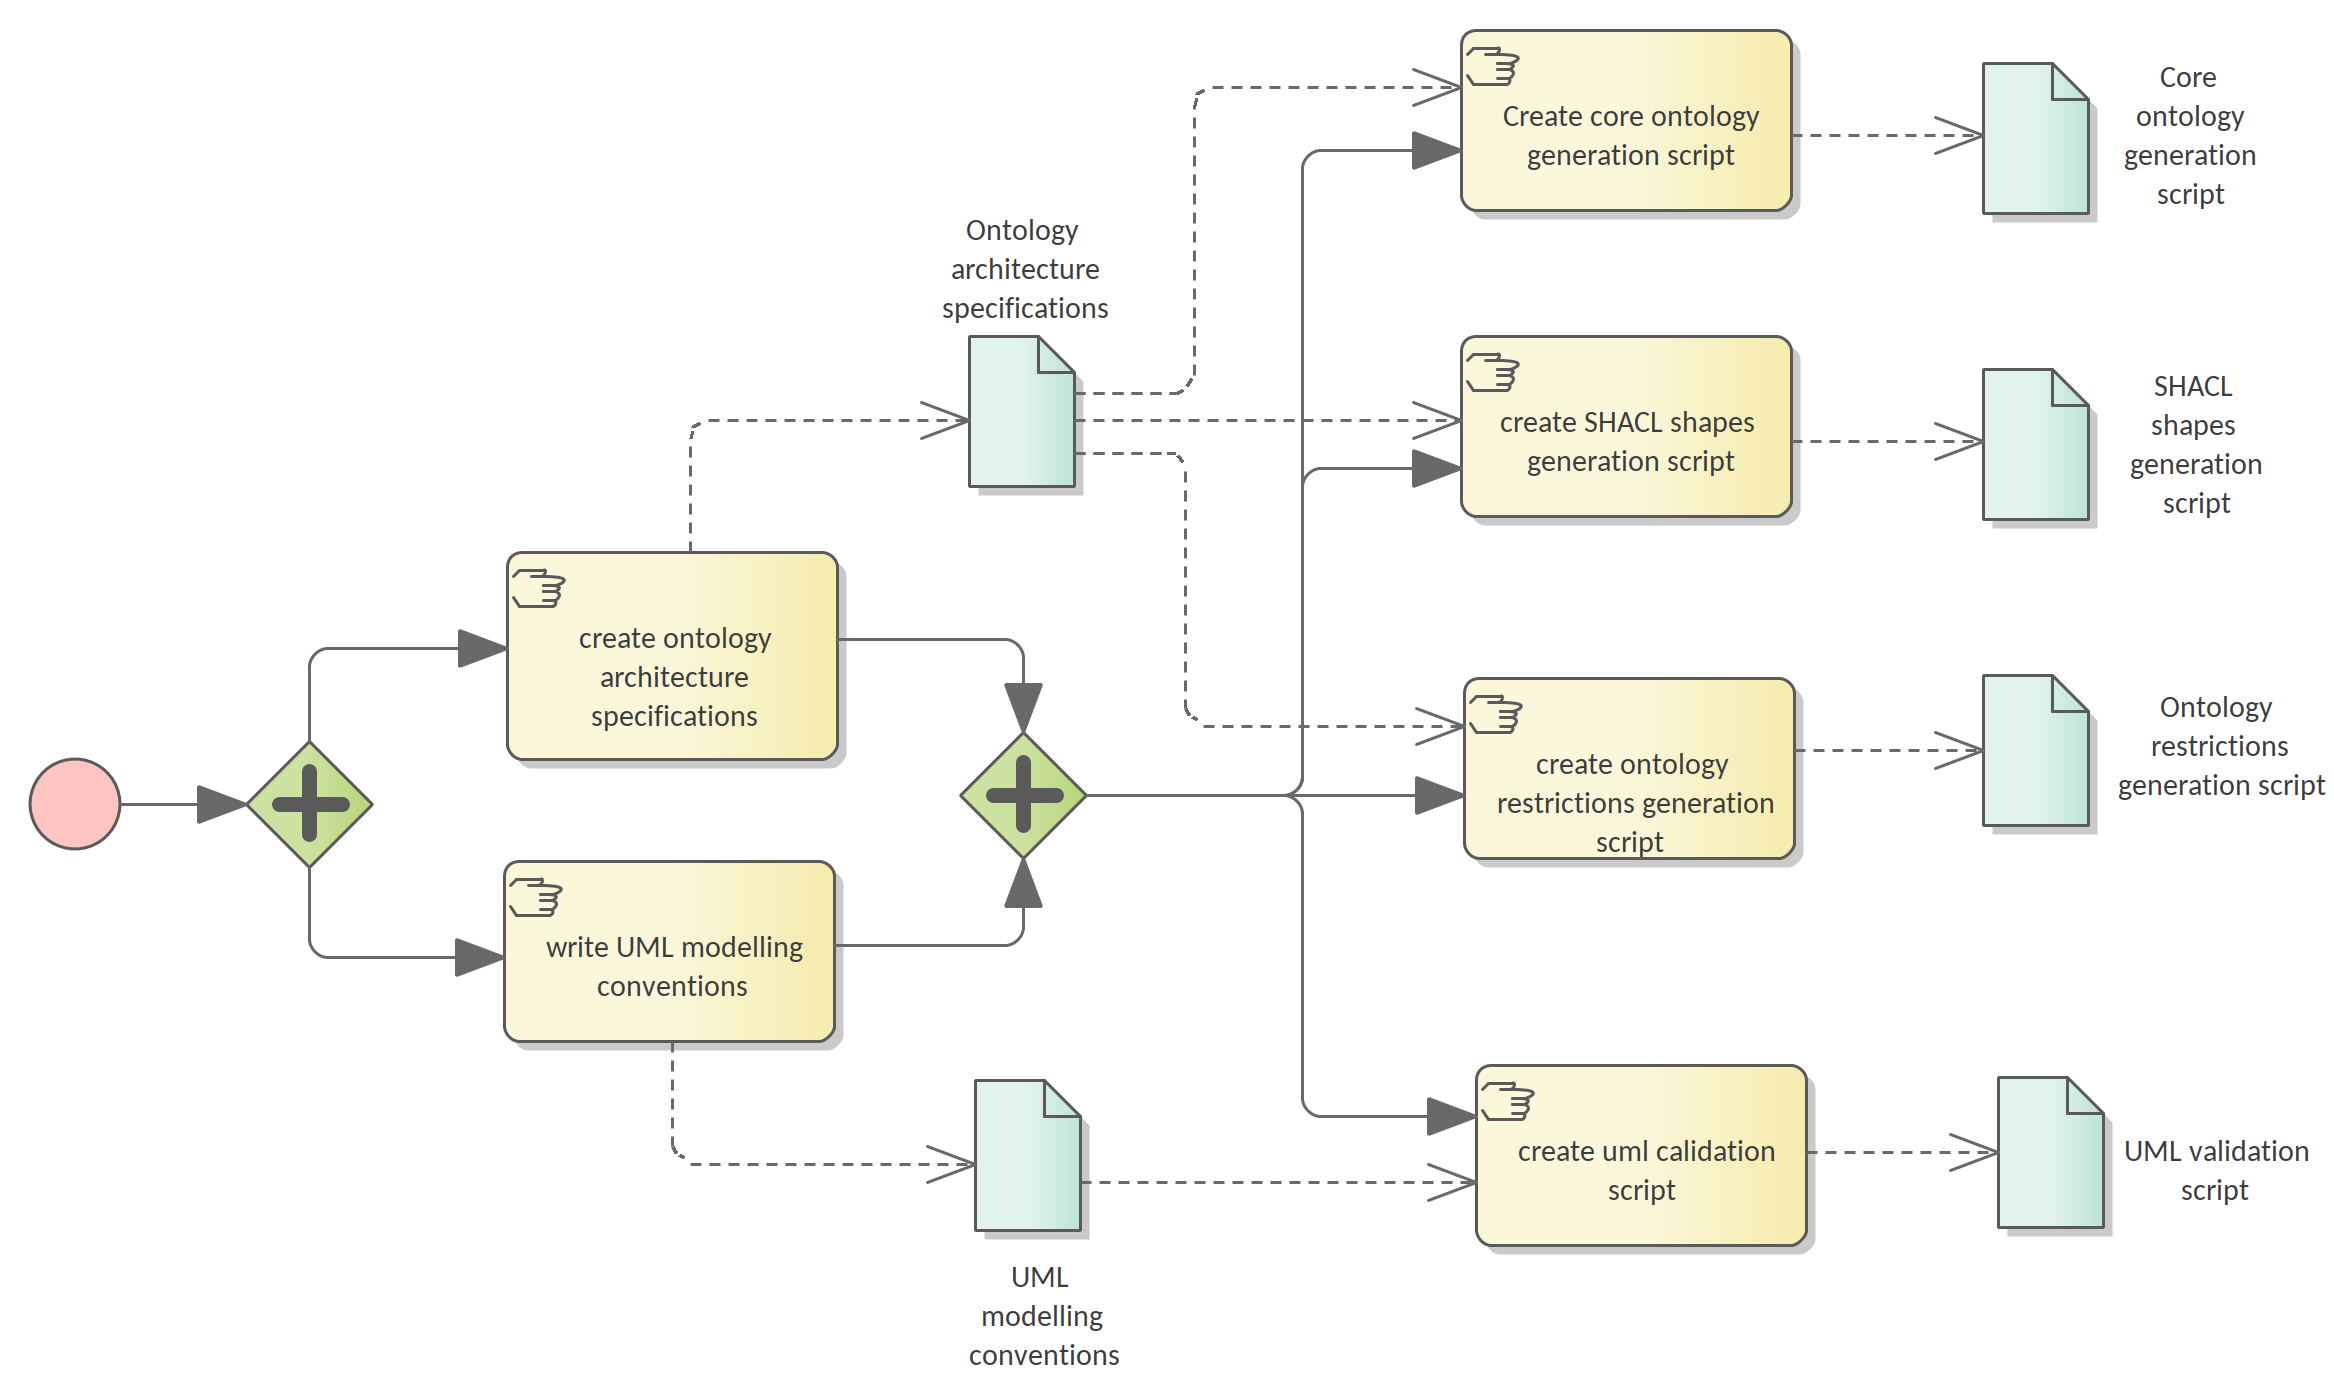
\includegraphics[width=\textwidth]{../img/uml2formalScriptCreation.png}
		\caption{Creation of the specifications documents and the UML transformation scripts}
		\label{fig:uml-transformation}
	\end{figure}
	
	The conceptual model must comply with a set of UML modelling conventions making it suitable input for the transformation scripts, which implement the same conventions. The two parallel actions staring the process are depicted in Figure \ref{fig:uml-transformation}.
		
	The UML conventions document serves, at large, as requirements specification for the XSLT script that checks the UML conceptual model  whether it conforms to the conventions.
	
	The ontology architecture specification (this document) serves, at large, as requirement specifications for the development of three XSLT scripts to generate the formal ontology. These scripts can be developed independent of each other as they refer to different aspects of the formal ontology as described in Section \ref{sec:separation-concerns}.
	
	The input for these scripts is the UML conceptual model serialised in XMI 2.5.1 format \cite{xmi2.5.1}.
	
	\subsection{Conceptual model revision}
	\label{sec:revision-cm}
	
	The conceptual model revision is an iterative process. The validation script is execution outputs a report indicating if there are any deviations from the conventions, and detailing which are they and eventually what are the necessary actions to resolve them. 
	
	\begin{figure}[!ht]	
		\centering
		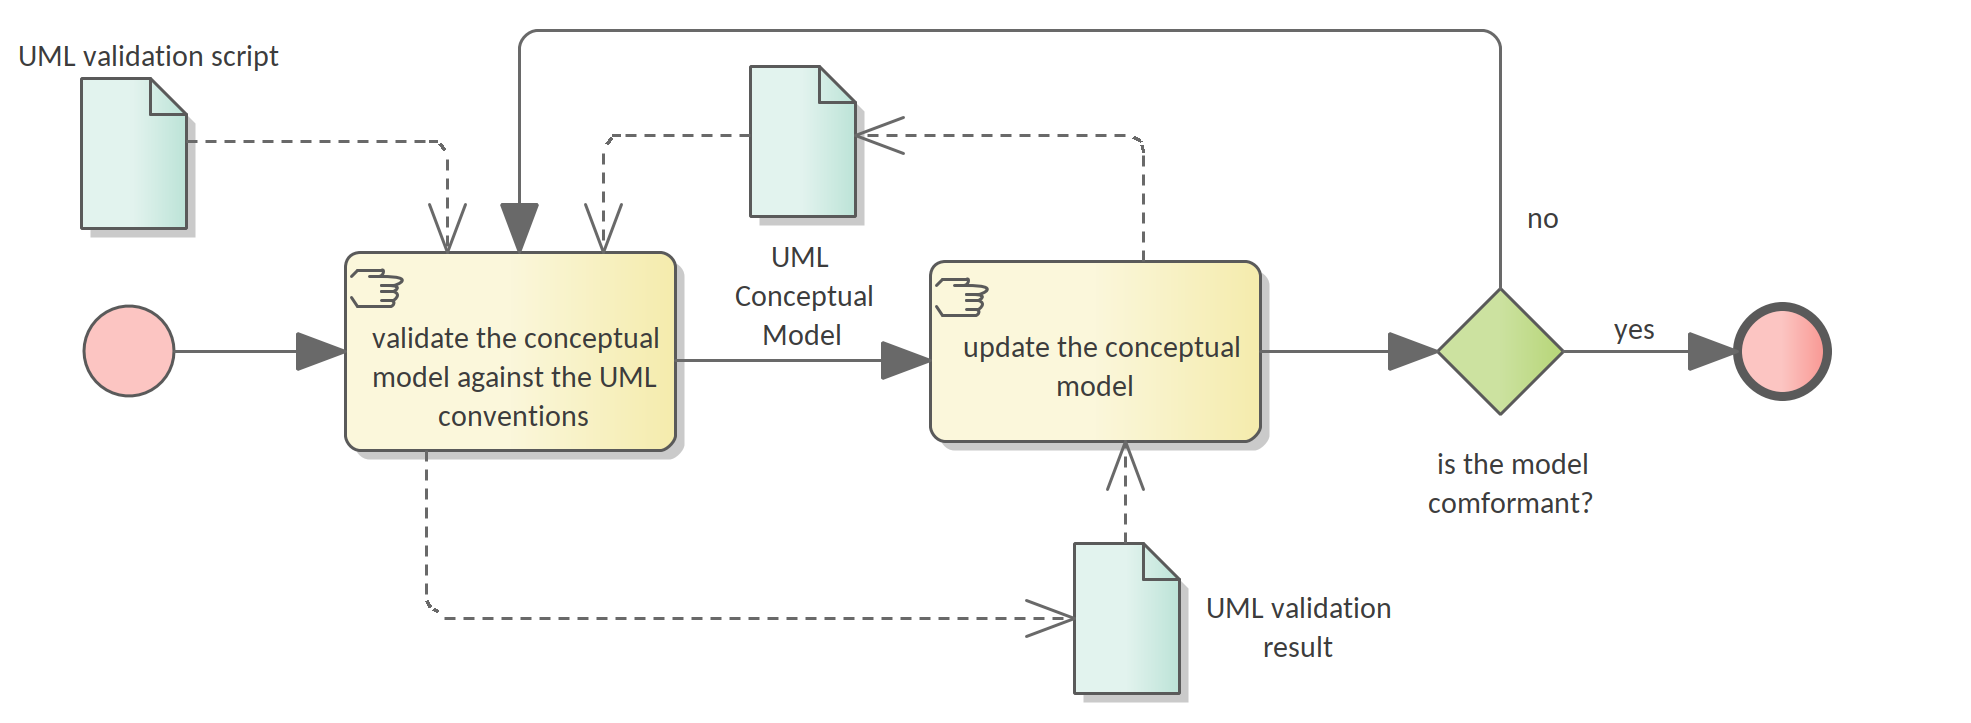
\includegraphics[width=.85\textwidth]{../img/conceptualModelRevision.png}
		\caption{Adjustment of the UML conceptual model guided by the validation script}
		\label{fig:revision-cm}
	\end{figure}
	
	\subsection{Formal ontology generation}
	\label{sec:ontology-generation}
	
	\begin{figure}[!ht]		
		\centering
		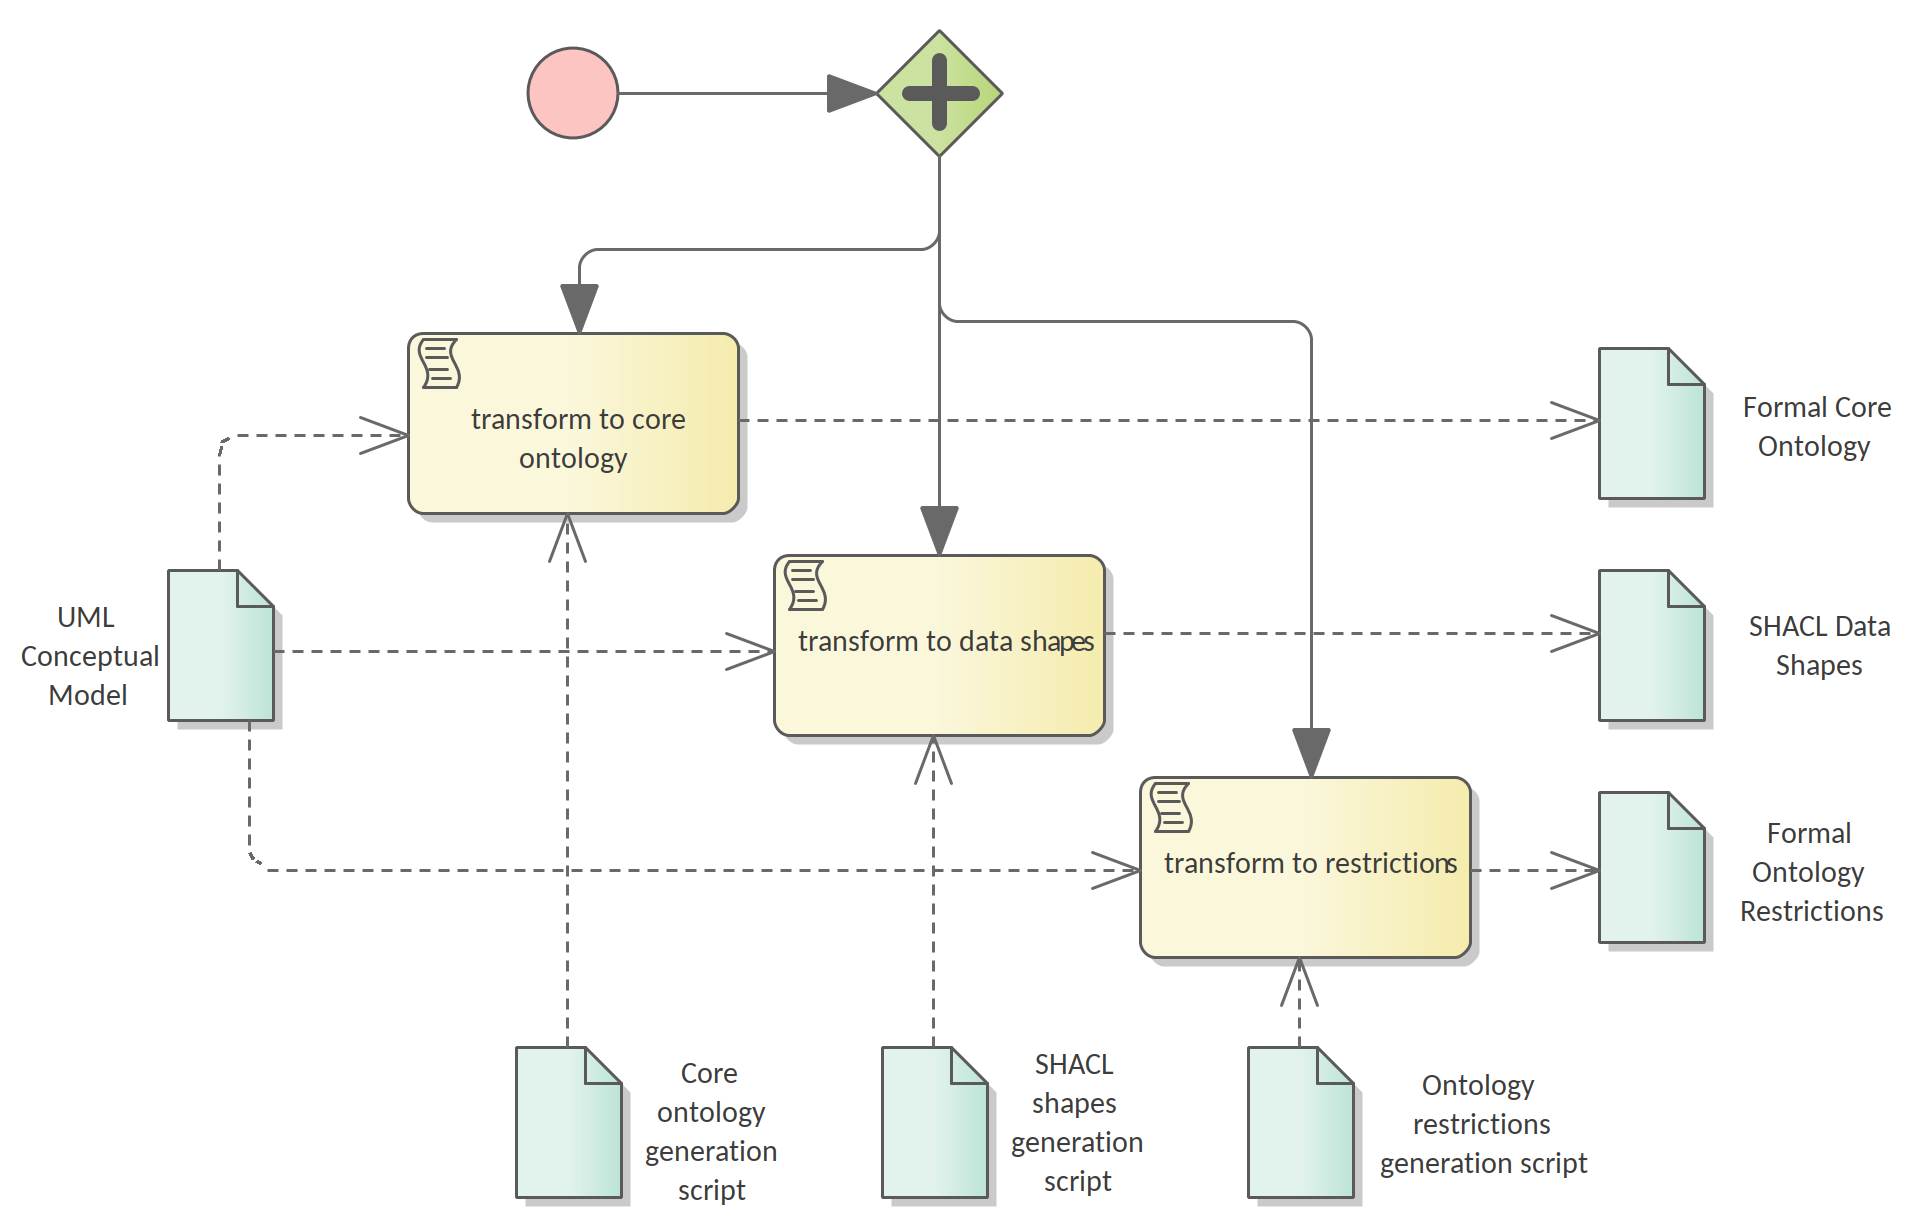
\includegraphics[width=\textwidth]{../img/formalOntologyGeneration.png}
		\caption{Generation of the formal ontology from the UML conceptual model}
		\label{fig:ontology-generation}
	\end{figure}
	

	\subsection{XML to RDF data transformation}
	\label{sec:xml2rdf}
	

	\begin{figure}
		\centering
		\begin{subfigure}[b]{.48\textwidth}
			\centering
			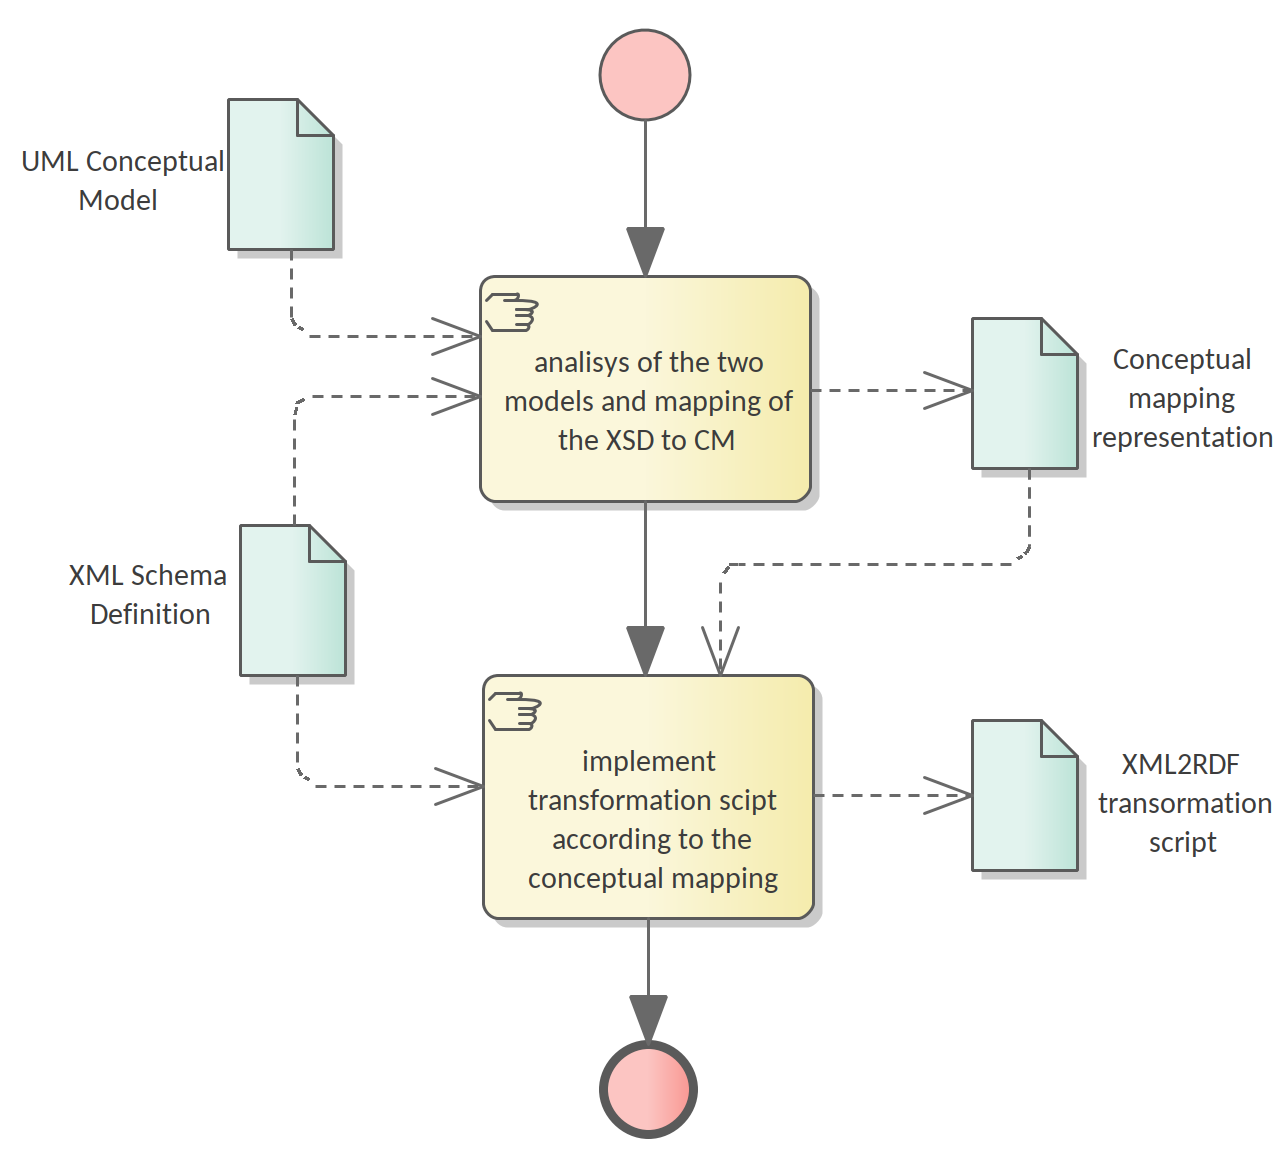
\includegraphics[width=1.05\linewidth]{../img/xml2rdfScriptCreation.png}
			\caption{Implementation of the XML transformations script based on the mappings from XSD schemas onto the conceptual model}
			\label{fig:sub1}
		\end{subfigure}%
		\quad
		\begin{subfigure}[b]{.48\textwidth}
			\centering
			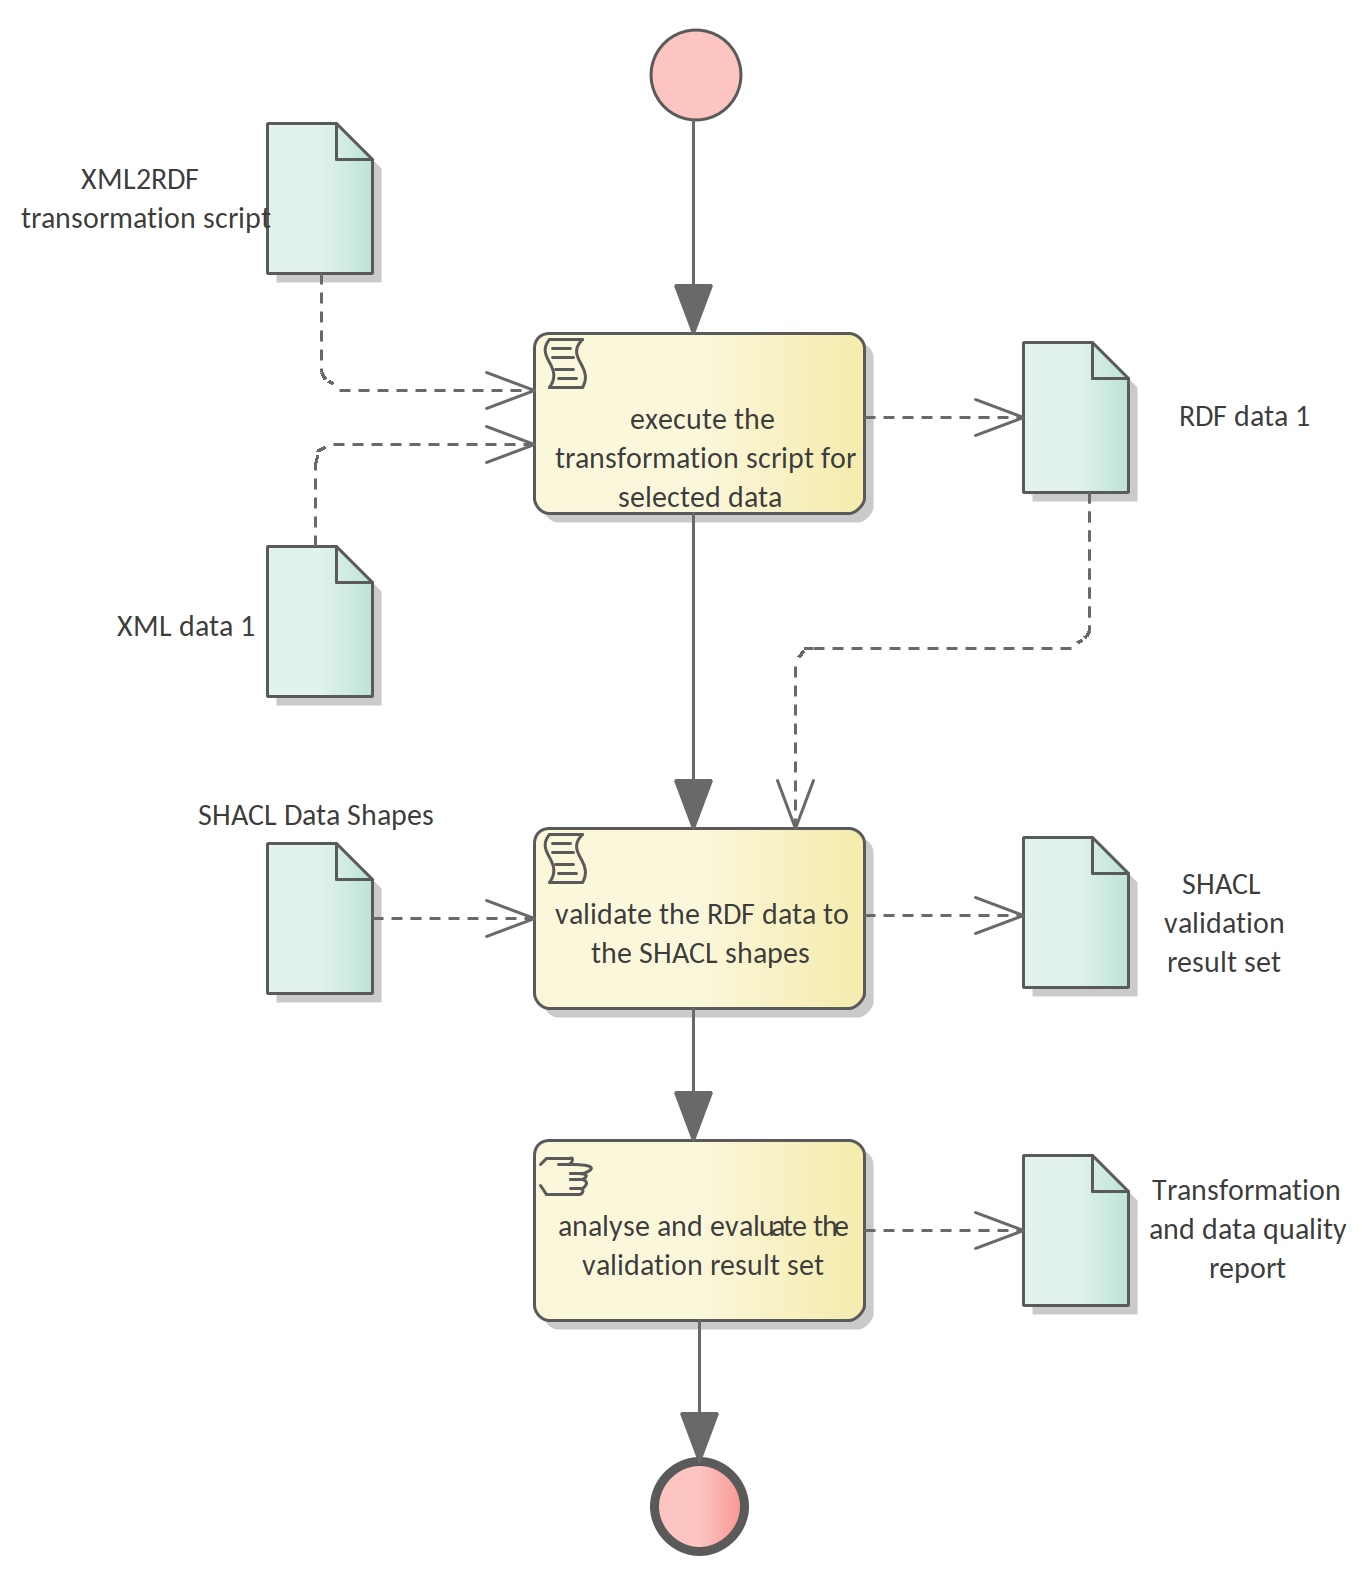
\includegraphics[width=1.05\linewidth]{../img/xmlDataTransformation.png}
			\caption{Transformation of the existent eProcurement XML data into RDF representation and validating the end result conformance}
			\label{fig:sub2}
		\end{subfigure}
		\caption{XML to RDF data transformation}
		\label{fig:test}
	\end{figure}

	
	